\documentclass[leqno]{article}
\usepackage[utf8]{inputenc}
\usepackage{enumitem}
\usepackage{tikz}
\usepackage[parfill]{parskip}
\usepackage{mathtools}
\usepackage{amsmath}
\usepackage{amssymb}

\title{Computationele logica}
\author{
    Kamans, Jim\\
    \texttt{10302905}
    \and
    Roosingh, Sander\\
    \texttt{11983957}
    \and
    Schenk, Stefan\\
    \texttt{11881798}
}
\date{November 2017}

\begin{document}

\maketitle

\textbf{Possibility:} $\sim_a \coloneqq \leq_a \cup \geq_a$

\textbf{Information Cell:} $w(a) \coloneqq \{s\in W:w\sim_a s\}$

\textbf{Knowledge:} $\lVert K_a \varphi \rVert_M = \{s\in W:s(a) \subseteq
\lVert \varphi \rVert_M\}$

\textbf{Conditional Belief:} $\lVert B_a^\varphi \psi \rVert_M = \{s \in
W:best_a(\lVert\varphi\rVert_M \cap s(a)) \subseteq \lVert\psi\rVert_M\}$ \\


%%%%%%%%%%%%%%%%
%% Exercise 1 %%
%%%%%%%%%%%%%%%%
\section*{Exercise 1}

\textit{(a) Show the following equivalence:}
\begin{center}
    $K_a \varphi \Leftrightarrow B_a^{\neg \varphi} false$
\end{center}

Take $s \in W$ such that $s \models_M K_a \varphi$ \textbf{(1)}.

Because \textbf{(1)} and \textbf{(Knowledge)} for all $t \in s(a)$ it's true
that: $t \models_M \varphi$ \textbf{(2)}.

Eliminating any world or all worlds either results in a world from s(a), where $K_a \varphi$, or no worlds at all, so $false$. \\
% TODO: Nog niet af


\textit{(b) Prove semantically the equivalence claimed on Slide 24 of Lecture
Notes 4.2:}
\begin{center}
    $B_a \phi \Leftrightarrow \lozenge_a \square_a \phi$
\end{center}
where $\Diamond a \phi : \neg \square a \neg \phi$ is the dual modality to safe
belief $\square a$.

[ANSWER HERE]

\textit{(c) Prove (via a counterexample) that safe belief does NOT imply strong
belief; i.e. that}
\begin{center}
    $\square_a \varphi \nRightarrow Sb_a \varphi$
\end{center}

[ANSWER HERE]

\textbf{HINT}: The positive statements (a) and (b) need general proofs: you
need to show that, for every plausibility model and every sentence $\phi$, the
desired formula is true at all the worlds of that model. But the negative
statement (c) must be shown by giving a counterexample: construct some
plausibility model and find some sentence $\varphi$ for which the implication
fails to be true at some world of that model (which we can think of as the
“real world”).

%%%%%%%%%%%%%%%%
%% Exercise 2 %%
%%%%%%%%%%%%%%%%
\pagebreak
\section*{Exercise 2}

% A virtual agent in a video game doesn’t know his current position in the
% virtual space, but all he cares is (a) whether or not he’s in a “Dangerous”
% zone (say, close to a dangerous monster).

% And (b) whether or not he’s close to his Target (say, a treasure). Let’s use
% the letter d to denote the sentence the agent is in a dangerous zone, and the
% letter t to denote the sentence the agent is close to the target.

% These possibilities are independent of each other, and the agent doesn’t know
% which is the case, so he cannot exclude any of the four possible cases d∧t,
% d∧¬t, ¬d∧t and ¬d∧¬t.

\begin{enumerate}
    \item \textit{Write down a logical formula in the language of beliefs,
    knowledge and conditional beliefs to encode all the above assumptions.}
    \[
    % However, our agent believes both that he’s close to the target AND that
    % he’s NOT in a dangerous zone.
        B_a(t \wedge \neg d) \wedge
    % If he would learn that this belief is WRONG (i.e. that at least one of
    % his two beliefs is false), then he’d still believe (conditional on this
    % new information) that he is close to the target.
    %    B_a^{ \neg (t \wedge \neg d)} t \wedge % EERSTE POGING
    % But if he would learn instead that he’s far from (=NOT close to) the
    % target, then (conditional on this information) he’d keep his initial
    % belief that he’s NOT in a dangerous zone.
    %   B_a^{(\neg t)} \neg d % EERSTE POGING
        B_a^{(t \wedge d)} (t \wedge d) \wedge
        B_a^{(\neg t \wedge \neg d)} (\neg t \wedge \neg d) \wedge
        B_a^{(\neg t \wedge d)} (\neg t \wedge \neg d)
    \]

    \item \textit{Represent the agent’s beliefs (and conditional beliefs),
    using a plausibility model with four possible worlds. Specify the valuation
    (which atomic sentences of the two atomic sentences d and t are true at
    which worlds). Represent the agent’s plausibility relation on these worlds,
    by drawing arrows going from the less plausible worlds to the more plausible
    ones.}

    \begin{center}
    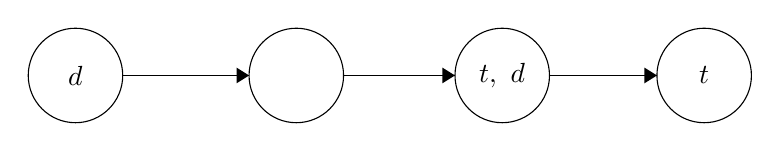
\begin{tikzpicture}[scale=0.2]
    \tikzstyle{every node}+=[inner sep=0pt]
    \draw [black] (51.233,-16.211) circle (3);
    \draw (51.23,-16.21) node {$t,\mbox{ }d$};
    \draw [black] (24.133,-16.211) circle (3);
    \draw (24.13,-16.21) node {$d$};
    \draw [black] (64.056,-16.211) circle (3);
    \draw (64.06,-16.21) node {$t$};
    \draw [black] (38.156,-16.211) circle (3);
    \draw [black] (54.23,-16.21) -- (61.06,-16.21);
    \fill [black] (61.06,-16.21) -- (60.26,-15.71) -- (60.26,-16.71);
    \draw [black] (27.13,-16.21) -- (35.16,-16.21);
    \fill [black] (35.16,-16.21) -- (34.36,-15.71) -- (34.36,-16.71);
    \draw [black] (41.16,-16.21) -- (48.23,-16.21);
    \fill [black] (48.23,-16.21) -- (47.43,-15.71) -- (47.43,-16.71);
    \end{tikzpicture}
    \end{center}

    \item \textit{Suppose somebody who never lies tells our agent “You are
    close to the target if and only if you believe that you are in a dangerous
    zone.” Write down formally this sentence as a formula $\varphi$ in doxastic
    logic (using the atomic sentences).}

    $\varphi \coloneqq t_a^{(B_a d)} \wedge B_a d^{(t_a)}$

    \item \textit{Interpreting the above truthful announcement $!\varphi$ as an
    update with the sentence $\varphi$ in the previous part, represent the
    updated model.}

    \begin{center}
    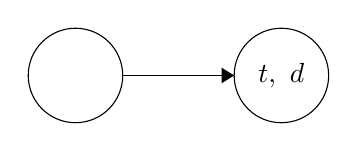
\begin{tikzpicture}[scale=0.2]
    \tikzstyle{every node}+=[inner sep=0pt]
    \draw [black] (51.233,-16.211) circle (3);
    \draw (51.23,-16.21) node {$t,\mbox{ }d$};
    % \draw [black] (24.133,-16.211) circle (3);
    % \draw (24.13,-16.21) node {$d$};
    % \draw [black] (64.056,-16.211) circle (3);
    % \draw (64.06,-16.21) node {$t$};
    \draw [black] (38.156,-16.211) circle (3);
    % \draw [black] (54.23,-16.21) -- (61.06,-16.21);
    % \fill [black] (61.06,-16.21) -- (60.26,-15.71) -- (60.26,-16.71);
    % \draw [black] (27.13,-16.21) -- (35.16,-16.21);
    % \fill [black] (35.16,-16.21) -- (34.36,-15.71) -- (34.36,-16.71);
    \draw [black] (41.16,-16.21) -- (48.23,-16.21);
    \fill [black] (48.23,-16.21) -- (47.43,-15.71) -- (47.43,-16.71);
    \end{tikzpicture}
    \end{center}

    \item \textit{After the previous announcement, another truthful
    announcement is made: “You are in a dangerous zone if and only if you don’t
    believe that you are in a dangerous zone.” Write down formally this
    sentence as a formula $\psi$ in doxastic logic (using the atomic
    sentences).}

    $\psi \coloneqq d_a^{(B_a \neg d_a)} \wedge B_a \neg d_a^{(d_a)}$

    \item \textit{What is the real world? (In other words, answer the question:
    is the agent in a dangerous zone or not, and is he close to the target or
    not?) Justify your answer, by interpreting the announcement in the previous
    part as a new update $\neg \psi$ and representing the updated model.}

    The agent believes that it's most plausible that he's in a dangerous zone,
    if $\neg \psi$, the agent knows that if he believes this, he's not in a
    dangerous zone.

    \begin{center}
    
\begin{tikzpicture}[scale=0.2]
    \tikzstyle{every node}+=[inner sep=0pt]
    % \draw [black] (51.233,-16.211) circle (3);
    % \draw (51.23,-16.21) node {$t,\mbox{ }d$};
    % \draw [black] (24.133,-16.211) circle (3);
    % \draw (24.13,-16.21) node {$d$};
    % \draw [black] (64.056,-16.211) circle (3);
    % \draw (64.06,-16.21) node {$t$};
    \draw [black] (38.156,-16.211) circle (3);
    % \draw [black] (54.23,-16.21) -- (61.06,-16.21);
    % \fill [black] (61.06,-16.21) -- (60.26,-15.71) -- (60.26,-16.71);
    % \draw [black] (27.13,-16.21) -- (35.16,-16.21);
    % \fill [black] (35.16,-16.21) -- (34.36,-15.71) -- (34.36,-16.71);
    % \draw [black] (41.16,-16.21) -- (48.23,-16.21);
    % \fill [black] (48.23,-16.21) -- (47.43,-15.71) -- (47.43,-16.71);
    \end{tikzpicture}
    \end{center}

\end{enumerate}

\end{document}
